\documentclass[border=6pt]{standalone}
% Shared preamble for web figures.  Each figure is a standalone .tex that
% \input's this file; scripts/make-figures.sh turns it into an SVG.
% Handouts pull the same file with \fig{Unit_X/<name>}.
\usepackage[T1]{fontenc}
\usepackage{helvet}
\renewcommand{\familydefault}{\sfdefault}
\renewcommand{\ttdefault}{pcr}  % Courier: a real Type 1 typewriter font
\usepackage{amsmath}
\usepackage{tikz}
\usetikzlibrary{arrows.meta,positioning,calc,shapes.symbols,shapes.geometric}

% Who makes the rules is the point of most diagrams in this book, so the
% colors mean the same thing everywhere: blue is a person, orange is the
% computer, green is an answer, pink is the human brain.
\definecolor{person}{HTML}{2C6FAE}
\definecolor{machine}{HTML}{D35400}
\definecolor{result}{HTML}{1E8449}
\definecolor{brainpink}{HTML}{C2185B}
\definecolor{ink}{HTML}{2C3E50}

\tikzset{
  doodle/.style={line width=1.5pt, line cap=round, line join=round, draw=ink},
  box/.style={draw, rounded corners=5pt, line width=1.1pt, align=center,
              inner sep=7pt, minimum height=1.0cm, font=\small},
  personbox/.style={box, draw=person, fill=person!10},
  machinebox/.style={box, draw=machine, fill=machine!10},
  resultbox/.style={box, draw=result, fill=result!10},
  plainbox/.style={box, draw=ink!70, fill=ink!4},
  flow/.style={-{Stealth[length=8pt]}, line width=1.4pt, draw=ink},
}

% A person (blue) and a robot head (orange) as small icons.
% \personicon{x}{y}{scale}   \roboticon{x}{y}{scale}
\newcommand{\personicon}[3]{%
  \begin{scope}[shift={(#1,#2)}, scale=#3]
    \fill[person] (0,0.62) circle (0.28);
    \fill[person, rounded corners=6pt] (-0.42,-0.55) rectangle (0.42,0.28);
  \end{scope}}
\newcommand{\roboticon}[3]{%
  \begin{scope}[shift={(#1,#2)}, scale=#3]
    \draw[machine, line width=1.2pt] (0,0.5) -- (0,0.72);
    \fill[machine] (0,0.78) circle (0.08);
    \draw[machine, line width=1.4pt, fill=machine!12, rounded corners=4pt] (-0.5,-0.45) rectangle (0.5,0.5);
    \fill[ink] (-0.2,0.12) circle (0.08);
    \fill[ink] (0.2,0.12) circle (0.08);
    \draw[ink, line width=1pt] (-0.22,-0.22) -- (0.22,-0.22);
  \end{scope}}

\usetikzlibrary{backgrounds}
\begin{document}
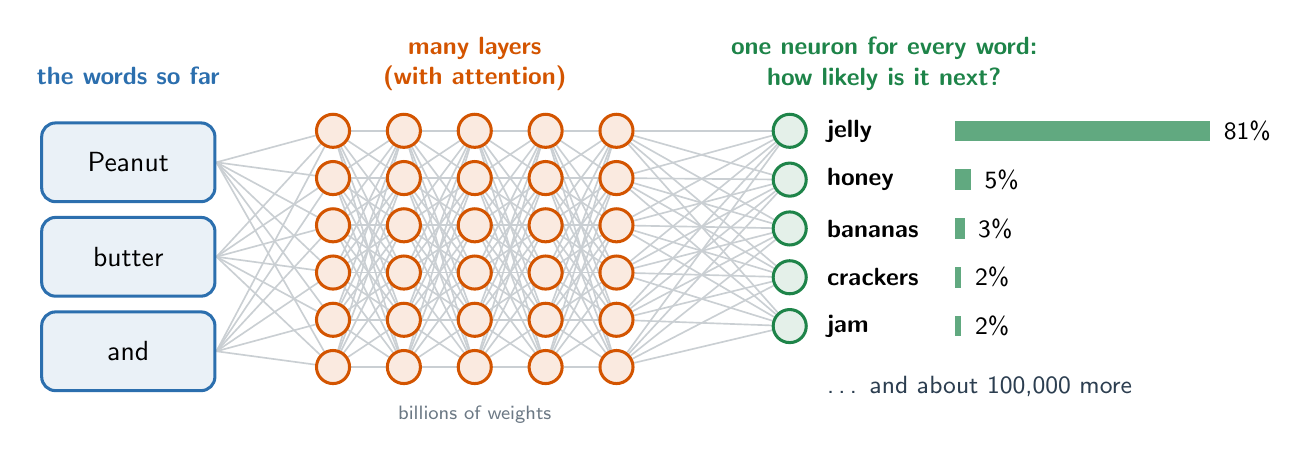
\begin{tikzpicture}[
  inp/.style={personbox, minimum width=2.2cm, font=\normalsize},
  hid/.style={circle, draw=machine, fill=machine!12, line width=1.1pt, minimum size=0.42cm, inner sep=0pt},
  wire/.style={draw=ink!25, line width=0.6pt},
]
% A real chatbot is a network. The words so far go in. Many layers. The
% output layer has one neuron for every word, each with a percentage.
% The percentages are made up to show the idea.
\node[inp] (w1) at (0,2.2) {Peanut};
\node[inp] (w2) at (0,1.0) {butter};
\node[inp] (w3) at (0,-0.2) {and};
\node[font=\small\bfseries, text=person, align=center] at (0,3.3) {the words so far};
\foreach \c in {0,...,4} \foreach \r in {0,...,5} \node[hid] (h\c-\r) at (2.6+\c*0.9, 2.6-\r*0.6) {};
\begin{scope}[on background layer]
  \foreach \i in {1,2,3} \foreach \r in {0,...,5} \draw[wire] (w\i.east) -- (h0-\r);
  \foreach \c [evaluate=\c as \n using int(\c+1)] in {0,...,3} \foreach \r in {0,...,5} \foreach \s in {0,...,5} \draw[wire] (h\c-\r) -- (h\n-\s);
\end{scope}
\node[font=\small\bfseries, text=machine, align=center] at (4.4,3.45) {many layers\\(with attention)};
\node[font=\scriptsize, text=ink!70] at (4.4,-1.0) {billions of weights};
% output layer: one neuron per word, with percentage bars
\foreach \w/\p/\r in {jelly/81/0, honey/5/1, bananas/3/2, crackers/2/3, jam/2/4} {
  \node[circle, draw=result, fill=result!12, line width=1.1pt, minimum size=0.42cm, inner sep=0pt] (o\r) at (8.4, 2.6-\r*0.62) {};
  \node[anchor=west, font=\small\bfseries] at (8.75, 2.6-\r*0.62) {\w};
  \fill[result!70] (10.5, 2.6-\r*0.62-0.13) rectangle ++(\p*0.04, 0.26);
  \node[anchor=west, font=\small] at (10.55+\p*0.04, 2.6-\r*0.62) {\p\%};
}
\node[font=\small, text=ink, anchor=west] at (8.75,-0.65) {\dots\ and about 100,000 more};
\begin{scope}[on background layer]
  \foreach \r in {0,...,5} \foreach \o in {0,...,4} \draw[wire] (h4-\r) -- (o\o);
\end{scope}
\node[font=\small\bfseries, text=result, align=center] at (9.6,3.45) {one neuron for every word:\\how likely is it next?};
\end{tikzpicture}
\end{document}
